% Capstone report: Mechanistic Analysis of Over-Squashing and Attention Dilution in Hybrid GNNs
% Formatting follows the MSADS "Capstone Proposal & Research Paper Guide 2025":
% Times 12pt, US letter, double spacing, unnumbered headings (L1 centred 14pt bold,
% L2 left 12pt bold, L3 left 12pt bold italic), captions above floats
% ("Figure 1." bold + italic description), roman front-matter pages, arabic from the
% Introduction, APA references.
% Build: latexmk -pdf main.tex   (figures are read from ./figures)
\documentclass[12pt,letterpaper]{article}

\usepackage[T1]{fontenc}
\usepackage[utf8]{inputenc}
\usepackage{newtxtext,newtxmath}
\usepackage[margin=1in]{geometry}
\usepackage{setspace}
\usepackage{amsmath}
\usepackage{graphicx}
\usepackage{booktabs}
\usepackage{array}
\usepackage{multirow}
\usepackage{float}
\usepackage{xcolor}
\usepackage{etoolbox}
\usepackage{pgfplots}
\usepgfplotslibrary{groupplots}
\pgfplotsset{compat=1.17}
\usepackage[titles]{tocloft}
\usepackage{titlesec}
\usepackage[font=normalsize,labelfont=bf,textfont=it,labelsep=period,
            justification=centering,singlelinecheck=false,position=top,skip=6pt]{caption}
\usepackage[round,authoryear]{natbib}
\usepackage[hidelinks]{hyperref}

\graphicspath{{figures/}}
\newcolumntype{L}[1]{>{\raggedright\arraybackslash}p{#1}}

% ---------------------------------------------------------------- spacing
\doublespacing
\setlength{\parindent}{0.5in}
\setlength{\parskip}{0pt}
% floats and the bibliography are single spaced so tables stay readable
\AtBeginEnvironment{table}{\singlespacing}
\AtBeginEnvironment{figure}{\singlespacing}
\setlength{\textfloatsep}{12pt plus 2pt minus 2pt}
\setlength{\intextsep}{12pt plus 2pt minus 2pt}

% ---------------------------------------------------------------- headings
\setcounter{secnumdepth}{0}
\setcounter{tocdepth}{2}
\titleformat{\section}{\centering\bfseries\fontsize{14}{17}\selectfont}{}{0pt}{}
\titleformat{\subsection}{\raggedright\bfseries\normalsize}{}{0pt}{}
\titleformat{\subsubsection}{\raggedright\bfseries\itshape\normalsize}{}{0pt}{}
\titlespacing*{\section}{0pt}{0pt}{0pt}
\titlespacing*{\subsection}{0pt}{0pt}{0pt}
\titlespacing*{\subsubsection}{0pt}{0pt}{0pt}

% ---------------------------------------------------------------- TOC and lists
\renewcommand{\cfttoctitlefont}{\hfill\bfseries\fontsize{14}{17}\selectfont}
\renewcommand{\cftaftertoctitle}{\hfill}
\renewcommand{\cftloftitlefont}{\hfill\bfseries\fontsize{14}{17}\selectfont}
\renewcommand{\cftafterloftitle}{\hfill}
\renewcommand{\cftlottitlefont}{\hfill\bfseries\fontsize{14}{17}\selectfont}
\renewcommand{\cftafterlottitle}{\hfill}
\setlength{\cftbeforetoctitleskip}{0pt}
\setlength{\cftbeforeloftitleskip}{12pt}
\setlength{\cftbeforelottitleskip}{12pt}
\setlength{\cftaftertoctitleskip}{6pt}
\setlength{\cftafterloftitleskip}{6pt}
\setlength{\cftafterlottitleskip}{6pt}
\renewcommand{\cftsecfont}{\normalfont}
\renewcommand{\cftsecpagefont}{\normalfont}
\renewcommand{\cftsecleader}{\cftdotfill{\cftdotsep}}
\setlength{\cftbeforesecskip}{0pt}
\setlength{\cftsecindent}{0pt}
\setlength{\cftsubsecindent}{0.5in}
\renewcommand{\cftfigpresnum}{\bfseries Figure~}
\renewcommand{\cftfigaftersnum}{.}
\renewcommand{\cfttabpresnum}{\bfseries Table~}
\renewcommand{\cfttabaftersnum}{.}
\setlength{\cftfignumwidth}{6.5em}
\setlength{\cfttabnumwidth}{6.5em}
\setlength{\cftfigindent}{0pt}
\setlength{\cfttabindent}{0pt}

% Appendix floats are numbered A1, A2, ... (guide: prefix with the appendix letter)
\newcommand{\appendixsection}[2]{%
  \section{Appendix #1: #2}%
  \setcounter{figure}{0}\setcounter{table}{0}%
  \renewcommand{\thefigure}{#1\arabic{figure}}%
  \renewcommand{\thetable}{#1\arabic{table}}}

\newcommand{\Hn}{\tilde{H}}

% ================================================================
\begin{document}

% ---------------------------------------------------------------- title page (no page number)
\begin{titlepage}
  \centering
  \vspace*{0.6in}
  {\fontsize{18}{22}\selectfont\bfseries Mechanistic Analysis of Over-Squashing and Attention Dilution in Hybrid Graph Neural Networks\par}
  \vspace{0.5in}
  {\fontsize{14}{17}\selectfont By\par}
  \vspace{0.15in}
  {\normalsize Collin McDevitt\par Dhawal Dixit\par Andy Jiang\par}
  \vspace{0.3in}
  {\normalsize Supervisor: Dr.\ Greg Green\par}
  \vspace{0.5in}
  {\fontsize{14}{17}\selectfont
   A Capstone Project\par
   \vspace{0.15in}
   Submitted to the University of Chicago in partial fulfillment\par
   of the requirements for the degree of\par
   \vspace{0.15in}
   Master of Science in Applied Data Science\par
   \vspace{0.15in}
   Division of Physical Sciences\par
   \vspace{0.3in}
   October 2026\par}
\end{titlepage}

% ---------------------------------------------------------------- front matter (roman)
\pagenumbering{roman}
\setcounter{page}{1}

\section*{Abstract}
\noindent Graph neural networks fail at long range in two ways: message passing over-squashes distant signals through bottlenecks, and global attention dilutes them across many nodes. We frame architecture choice as a blend weight $\alpha$ between the two and measure both mechanisms with effective resistance, Jacobian sensitivity, attention entropy and range. In river forecasting, an attention-heavy blend cut error by 9.6\% against message passing when only weather was observed, but gave no gain once flow history was supplied. A controlled tree task showed the same reach failure. The rebuilt Peptides-func hybrid reached 0.626 test average precision, short of its 0.652 calibration gate.

\vspace{1in}
\noindent\textit{Keywords:} graph neural networks, over-squashing, attention dilution, effective resistance, Jacobian sensitivity, graph transformers, hybrid architectures, long-range graph benchmark, hydrological forecasting

\newpage
\section*{Executive Summary}
Practitioners choose between message-passing graph neural networks, graph transformers and hybrids by training all three, which is costly and explains nothing. Message passing loses distant information at structural bottlenecks (over-squashing); global attention reaches every node but can spread its weight too thinly (attention dilution). We place every model on one axis, a blend weight $\alpha$ from pure message passing ($\alpha=0$) to pure attention ($\alpha=1$), and ask whether graph structure and task range predict the best $\alpha$.

Global access helped when the task needed information the local model could not use. On river discharge forecasting with weather inputs, $\alpha=0.75$ cut held-out error by 9.6\% against message passing, but beat pure attention and simple upstream pooling by only about 1\%. With discharge history as input, no blend beat message passing. On synthetic trees, message passing failed a four-hop query inside its receptive field, while every blend solved it. Upstream graph growth did not predict the hybrid's gain.

We measured the mechanisms with effective resistance, Jacobian sensitivity, normalized attention entropy and a range measure, and rebuilt the pilot pipeline after finding that its mechanistic results came from attention models that had not trained. The rebuilt Peptides-func hybrid reached 0.626 test average precision, below its 0.652 calibration gate, with signs of overfitting.

We recommend testing whether a task needs distant information, for example by hiding distant inputs, before paying the roughly 1.5-fold training cost of a hybrid. Next steps are to close the calibration gap, run the Peptides-func re-baseline with confidence intervals, sweep $\alpha$, and build the synthetic suite for a phase diagram of best $\alpha$ against effective resistance and task range.

\newpage
\begingroup
\singlespacing
\renewcommand{\contentsname}{Table of Contents}
\tableofcontents
\listoffigures
\listoftables
\endgroup

% ---------------------------------------------------------------- main text (arabic)
\newpage
\pagenumbering{arabic}
\setcounter{page}{1}

\section{Introduction}
Graph neural networks are the standard tool for learning on relational data such as molecules, social networks, transport systems and river networks. In each of these settings the prediction for one entity can depend on entities several steps away in the graph. Whether a model can use that distant information depends on how information moves through the architecture, and the two dominant architectures move it in opposite ways. A message-passing network moves information one edge per layer, while a graph transformer lets every node attend to every other node in a single layer. Hybrid models combine both, but there is still no principled way to decide in advance which of the three a given graph and task need.

\subsection{Problem Statement}
Current practice in applied graph learning is empirical: practitioners train a local message-passing model, a graph transformer and a hybrid such as GPS \citep{rampasek2022}, then select the configuration with the best validation score. This costs several full training runs per task and leaves the reason for the winner unexplained. The cost of the procedure grows with every new dataset, and its outcome does not transfer, because a validation score on one graph says nothing about the next.

The difficulty is that long-range graph learning is limited by at least two different mechanisms. Over-squashing occurs when information from exponentially many distant nodes must be compressed into fixed-size node states at a structural bottleneck \citep{alon2021,topping2022}. Effective resistance measures how hard it is for two nodes to communicate through the graph and bounds this effect \citep{digiovanni2023,black2023}. Attention dilution is the complementary failure of global attention: a softmax over $N$ nodes that does not concentrate gives each node a weight near $1/N$, so a relevant node's signal shrinks as the graph grows \citep{xing2024}. Benchmark results add to the confusion. Carefully tuned message-passing models close most of the reported gap between message passing and transformers on the Long Range Graph Benchmark \citep{tonshoff2024}, and recent work suggests that the benchmark's Peptides tasks are short-range in the first place \citep{bamberger2025}.

A practitioner would benefit from a diagnostic that, before or after a single training run, states which constraint binds on their graph and task. Such a diagnostic would reduce the number of architectures that must be trained, would explain failures instead of only ranking models, and would indicate when the extra cost of a hybrid is justified.

\subsection{Research Goals}
The project builds a quantitative framework that maps graph structure and task properties to a position on the local-to-global spectrum. We represent that position by a single blend weight $\alpha$ in each layer, from $\alpha=0$ (pure message passing) to $\alpha=1$ (pure attention). The framework has three components. The first is a set of mechanistic measurements computed on trained models: Jacobian sensitivity against effective resistance for over-squashing, normalized per-head attention entropy for dilution, and the range measure of \citet{bamberger2025} for how far a model's predictions actually reach. The second is a set of controlled comparisons across $\alpha$, with confidence intervals, on real and synthetic graphs. The third is a phase diagram with effective resistance on one axis and task range or dilution exposure on the other, coloured by the best $\alpha$, together with a simple predictor of the best $\alpha$.

Four hypotheses guide the work. (H1) At $\alpha=0$, Jacobian sensitivity decays with effective resistance more steeply than for the transformer, with hybrids in between. (H2) Normalized attention entropy rises with graph size in attention models. (H3) Peptides-func is a short-range task, so the best $\alpha$ on it will be low. (H4) The best $\alpha$ increases with effective resistance and with task range.

\subsection{Scope}
The study compares local, global and hybrid models built from one shared layer, so that only $\alpha$ changes between them. The main hybrid uses a GINE message-passing branch \citep{hu2020} and multi-head self-attention; GPS-style hybrids \citep{rampasek2022} are the reference design, and sparse or structured attention models such as Exphormer \citep{shirzad2023} and GRIT \citep{ma2023} are discussed but not trained. The real-data evaluation covers Peptides-func and Peptides-struct from the Long Range Graph Benchmark \citep{dwivedi2022}, a Reddit hyperlink graph \citep{kumar2018} for node-level regression, and LamaH-CE river gauge networks \citep{klingler2021} for discharge forecasting. Synthetic rooted trees provide controlled tests. All models respect the benchmark's 500,000-parameter budget on Peptides and were trained on a single GPU (a Colab T4 or a laptop RTX 3080), which rules out large foundation models and exhaustive hyperparameter searches. Findings are specific to these graph families; molecular graphs and river networks are near-trees, so they cannot separate effective resistance from hop distance, which is the role of the planned synthetic suite.

% ================================================================
\section{Background}
Graph neural networks compute a representation for each node by repeatedly combining it with information from other nodes. In the message-passing framework \citep{gilmer2017}, each layer updates a node from an aggregate of its neighbours' states, so after $L$ layers a node has seen exactly its $L$-hop neighbourhood. Graph convolutional networks \citep{kipf2017}, GraphSAGE \citep{hamilton2017} and the graph isomorphism network \citep{xu2019} are standard instances, and GINE extends the last of these with edge features \citep{hu2020}. A graph transformer instead applies self-attention \citep{vaswani2017} over all nodes of a graph, so every pair of nodes can exchange information in one layer, and it relies on positional or structural encodings to recover the graph structure that attention ignores \citep{dwivedi2021,ying2021,kreuzer2021}.

Two quantities recur throughout this report. The effective resistance $R(u,v)$ between nodes $u$ and $v$ is the electrical resistance between them when every edge is a unit resistor; it is small when many short paths connect the nodes and large when they are joined through a bottleneck, and on a tree it equals the hop distance. The Jacobian sensitivity $J(u,v)=\lVert\partial h_v^{(L)}/\partial h_u^{(0)}\rVert$ measures how much the final representation of node $v$ changes when the input at node $u$ changes, and so how much information from $u$ can reach $v$.

\subsection{Literature Review}
The bottleneck view of long-range failure began with \citet{alon2021}, who showed that message-passing networks struggle when a node must summarise exponentially many distant nodes in a fixed-width vector and named the effect over-squashing. \citet{topping2022} tied over-squashing to negatively curved edges and proposed rewiring the graph to relieve them. \citet{digiovanni2023} bounded the Jacobian sensitivity between two nodes in terms of network width, depth and graph topology, and \citet{black2023} showed that total effective resistance bounds over-squashing, which makes resistance a structural predictor that can be computed from the graph Laplacian before any model is trained. \citet{mishayev2025} argued that over-squashing can arise even between nearby nodes and separated bottleneck effects from vanishing gradients. These results describe a model class rather than a trained model, which is why this project measures the Jacobian of trained networks directly.

Graph transformers were developed in part to remove the bottleneck by giving every node direct access to every other node. Early work generalised the transformer to graphs with Laplacian positional encodings \citep{dwivedi2021}, Graphormer added degree and shortest-path encodings and performed strongly on molecular benchmarks \citep{ying2021}, and spectral attention made positional encodings learnable \citep{kreuzer2021}. GPS combined a message-passing layer and a global attention layer in every block and organised the design space of encodings and attention mechanisms \citep{rampasek2022}. Sparse alternatives such as Exphormer reduce the quadratic cost of attention with expander graphs \citep{shirzad2023}, while GRIT showed that strong graph inductive biases can be built into attention without message passing \citep{ma2023}.

The case for attention on long-range tasks rests largely on the Long Range Graph Benchmark \citep{dwivedi2022}, whose Peptides datasets were designed to need long-range interactions. \citet{tonshoff2024} showed that much of the reported advantage of transformers on this benchmark disappears when message-passing baselines are tuned with the same care, raising a GCN on Peptides-func from about 0.59 to about 0.69 average precision. \citet{bamberger2025} then proposed a model-based range measure, the influence-weighted mean distance between a node and the inputs that affect it, and found that models trained on the Peptides tasks use mostly short-range information. Together these results change the question from whether attention helps on average to when attention provides a benefit that message passing cannot.

Attention dilution is less established in graph learning than over-squashing but has a clear analogue in language models, where accuracy drops when relevant content sits in the middle of a long context \citep{liu2024}. In graphs, \citet{xing2024} described over-globalizing, in which global attention places substantial weight on distant and irrelevant nodes and hurts accuracy, and \citet{sun2025} related a similar over-aggregation effect to the number of nodes attention must cover. Capacity-controlled and gated global attention has been proposed as a remedy \citep{liu2026}. The entropy of a node's attention distribution, normalised by $\log N$, is the natural diagnostic: a value near one means attention is close to uniform and the model is exposed to dilution.

Graph neural networks have also been applied well outside molecular and social data. In hydrology, recurrent networks trained on large samples of catchments forecast river discharge competitively with conceptual models \citep{kratzert2019}, and gauge networks form directed trees in which upstream information flows to an outlet. River networks are therefore a natural real-world test of whether distant upstream information is used, with the Nash--Sutcliffe efficiency \citep{nash1970} as the domain's standard skill score. Finally, \citet{bamberger2025} and the benchmark of \citet{miglior2025} call for tasks with a known long-range dependency, which motivates the synthetic suite in this project.

% ================================================================
\section{Data}
The study uses four data sources that cover different regimes of graph size, task level and range (Table~\ref{tab:datasets}). Peptides-func is the main benchmark for the mechanistic measurements. The Reddit graph provides a single large graph with node-level targets. The river networks provide real directed trees in which the relevant information is known to flow from upstream. Synthetic trees provide tasks whose range is set by construction.

\begin{table}[htbp]
\caption{Datasets used in the study}
\label{tab:datasets}
\centering\small
\begin{tabular}{@{}L{1.45in}L{1.5in}L{1.45in}L{1.25in}@{}}
\toprule
Dataset & Graphs & Task & Metric \\
\midrule
Peptides-func (LRGB) & 15,535 molecules, about 151 nodes each & 10-label graph classification & Macro average precision \\
Peptides-struct (LRGB) & Same graphs & 11-target graph regression & Mean absolute error \\
Reddit hyperlinks (SNAP) & One graph, 35,776 subreddits & Node regression & MSE by hop band \\
LamaH-CE rivers & 32 gauge trees, 5--35 nodes & Discharge 1, 3 and 7 days ahead & NRMSE, NSE \\
Synthetic trees & 96 trees, 63 or 127 nodes & Near or far marked-value query & MSE \\
\bottomrule
\end{tabular}
\end{table}

\subsection{Data Sources}
Peptides-func and Peptides-struct come from the Long Range Graph Benchmark \citep{dwivedi2022}. Both contain the same 15,535 peptide molecular graphs, with on average about 151 nodes, 307 edges and a diameter of about 57. Nodes are atoms described by nine categorical columns, and edges are bonds described by three categorical columns. Peptides-func labels each graph with ten binary functional classes and is evaluated by macro average precision (AP); Peptides-struct assigns eleven continuous structural targets and is evaluated by mean absolute error. We used the standard split of 10,873 training, 2,331 validation and 2,331 test graphs. Because the two datasets share their graphs, any difference in the range a model uses between them must come from the task rather than the structure, which is how the task-range axis of the phase diagram is defined.

The Reddit graph is built from the Stanford Network Analysis Project (SNAP) hyperlink network \citep{kumar2018}, in which a node is a subreddit and a directed edge records a post in one subreddit that links to another. The body-hyperlink network has 35,776 nodes and 286,561 directed edges, which we used as an undirected graph for message passing. Each hyperlinking post carries 86 numeric properties, including character and word counts, sentiment scores and LIWC psycholinguistic categories, and node features are the mean of these properties over a subreddit's outgoing posts. Of the 35,776 nodes, 7,913 have no outgoing posts and therefore no features; they relay messages but are never supervised. The pilot target was the first property, character count, which ranges from 49 to 40,276. Train, validation and test nodes were defined by breadth-first-search distance from the subreddit with the highest out-degree: nodes within one hop (1,455) were used for training, nodes at two hops (17,876) for validation and nodes at three or more hops (7,939) for testing.

The river data come from LamaH-CE, a large-sample hydrology dataset for Central Europe \citep{klingler2021}. For each outlet gauge we extracted the directed tree of upstream gauges, giving 32 graphs with 5 to 35 nodes and depths of 1 to 8 hops. Twenty-seven development outlets fall in three hydrological dependency groups and five held-out outlets fall in four groups; the selected node sets do not overlap, but two held-out outlets share a dependency group through transfer links. Each node carries 90 days of daily inputs, and the target is outlet discharge 1, 3 and 7 days ahead. We used two input regimes: weather only, and weather plus historical discharge. Data were split by time, with 1981--1999 for training, 2000--2005 for validation and 2006--2017 for testing.

The synthetic trees are rooted trees with 63 or 127 nodes and a maximum root distance of 4 or 8 hops, generated under early, uniform and late growth profiles (where most nodes sit near the root, evenly spread, or far from it). The root always has exactly four children and no node has more than four. In each example every node carries an independent standard-normal value, four nodes at one hop and four at four hops are marked, and a query at the root asks for the scaled sum of either the near or the far marked set. The design comprises 96 unique trees (24 training, 24 validation and 48 test), with isomorphic duplicates rejected within and across splits. A small synthetic molecule-like dataset with 8 to 30 nodes, using the Peptides schema, served only for software tests.

\subsection{Descriptive Analysis}
Three properties of the data shape the analysis. First, the Peptides graphs are near-trees: almost every pair of atoms is joined by a single path, so effective resistance and hop distance are nearly collinear. A claim that resistance predicts over-squashing better than hop distance therefore cannot be tested cleanly on Peptides, and the size of a graph is also correlated with its mean resistance. All Peptides analyses report this collinearity, and size-controlled regressions are used wherever resistance is related to a model measurement.

Second, the pilot Reddit target was a poor test of long-range learning. Character count spans almost three orders of magnitude and is close to a deterministic function of other properties of the same subreddit's posts, such as word counts. A model can predict it almost entirely from a node's own features, so a gain from long-range information is not expected. The distance-based split also places test nodes farther from the training region than validation nodes, so a gain at far hop bands confounds reach with distribution shift. These observations motivated the target-selection procedure and the random-split control described in the Methodology.

Third, the river graphs are small and their structural descriptors move together. Across the 32 graphs the Spearman correlation between node count and depth is about 0.83 and between node count and drainage area about 0.77. We summarised each outlet's upstream structure by the growth profile $V(r)$, the number of upstream gauges within $r$ directed hops including the outlet itself (Figure~\ref{fig:growth}). Profiles that rise steeply reach many upstream nodes within a few hops, while slow profiles hold the same nodes at longer distances. Because $V(r)$ saturates at the graph size, large-radius values largely restate size.

\begin{figure}[htbp]
\caption{Upstream growth profiles $V(r)$ of the river gauge networks}
\label{fig:growth}
\centering
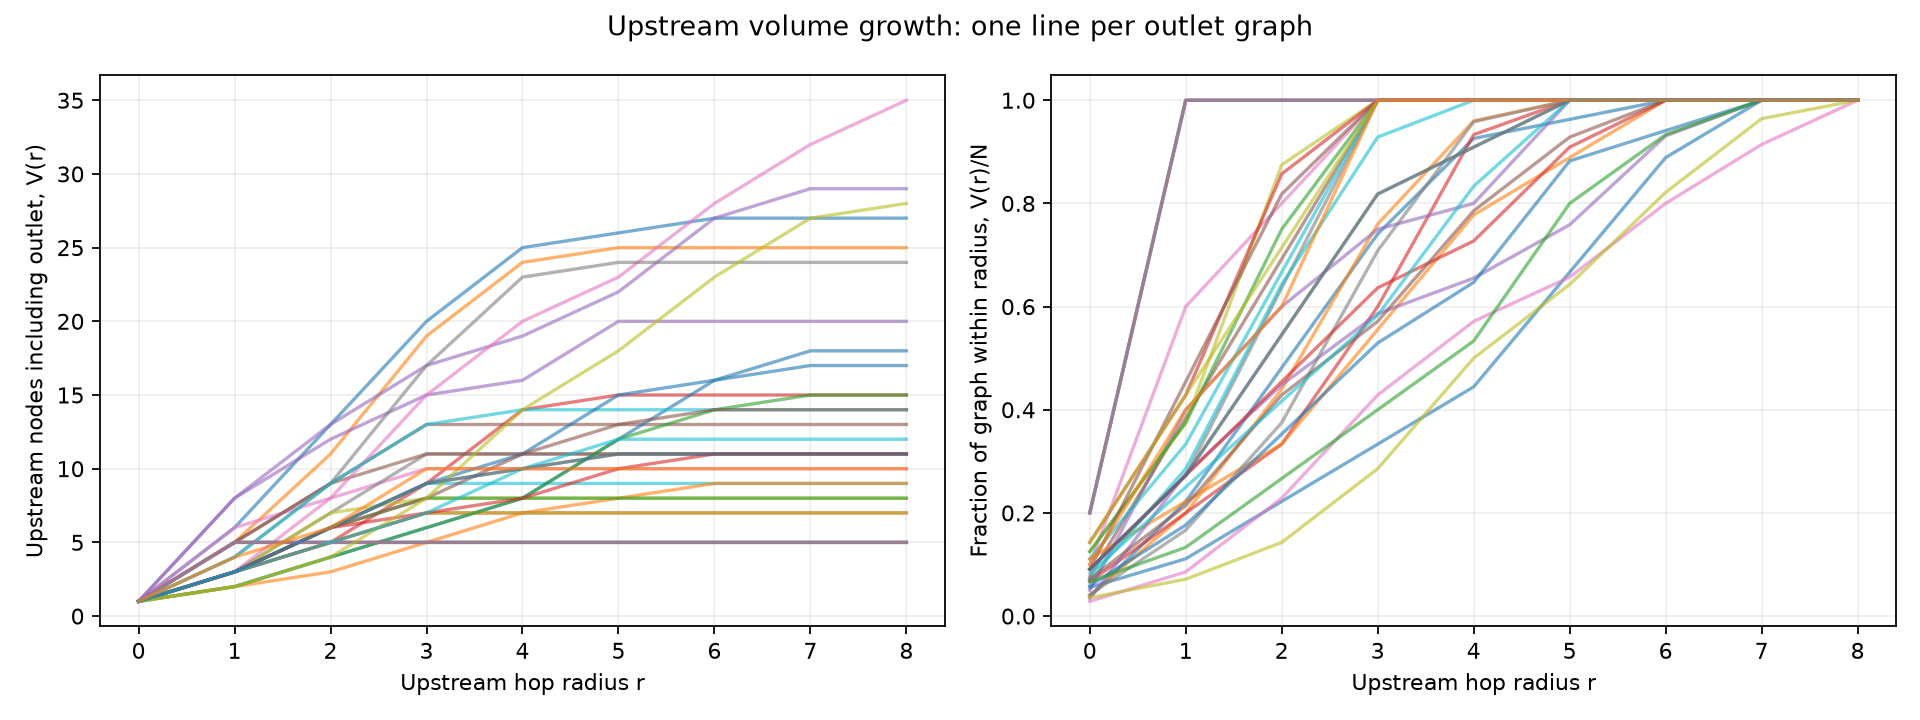
\includegraphics[width=0.85\textwidth]{river_upstream_growth_profiles.png}
\end{figure}

% ================================================================
\section{Methodology}
The methodology follows three principles. Every architecture is an instance of one layer with a blend weight $\alpha$, so that comparisons change one quantity at a time. Performance is stratified by structural difficulty rather than reported only as an aggregate. Mechanisms are measured directly on trained models, and every claim is preceded by a gate that checks the training regime is sound. We rebuilt the pilot code as a tested Python package, \texttt{gnn\_mech}, after a review found that the pilot mechanistic notebook had trained its models for only 30 epochs on one seed, passed categorical atom codes through a linear layer instead of embedding them, used no positional encoding, and averaged attention over heads before computing entropy.

\subsection{Feature Engineering}
For Peptides, each of the nine atom columns and three bond columns was embedded with its own learned lookup table using the Open Graph Benchmark vocabularies, and the column embeddings were summed into a node or edge vector of the model's hidden width. We added a random-walk structural encoding (RWSE) with 20 steps, $\mathrm{pe}_v=[(D^{-1}A)^k_{vv}]_{k=1}^{20}$, the probability that a random walk returns to its start after $k$ steps, projected linearly and added to the atom embedding to form the input $h_0$. All models received the same encoder. The dependent variables were the ten binary function labels. For each graph we cached its size, diameter and effective resistances, computed on the largest connected component as $R(u,v)=(e_u-e_v)^\top L^{+}(e_u-e_v)$ with $L=D-A$ and $L^{+}$ obtained from $(L+\tfrac1n\mathbf{1}\mathbf{1}^\top)^{-1}$.

For Reddit, standardisation used training-node statistics only, and input columns with an absolute correlation above 0.9 with the target were removed to exclude near-duplicates of it. Skewed non-negative targets were modelled on a $\log(1+y)$ scale. To choose a target that actually depends on the neighbourhood, we ranked candidate columns (sentiment and LIWC categories) on a random node split by how much ridge regression improved when a node's own features were augmented with the mean features of its 1- to 4-hop neighbourhoods, in the style of simplified graph convolution. A column was preferred when it showed clear multi-hop gain and moderate own-feature fit.

For the rivers, each node received daily weather series (and, in the second regime, discharge history) over a 90-day window together with static catchment attributes. Error was normalised by the development-period standard deviation of specific discharge scaled to each outlet's drainage area (NRMSE), so that outlets of different size contribute comparably. For the synthetic trees, each node received its value, a marked-node flag, a root flag and the root query, with no node identifier or depth feature. The target, the sum of the four requested values divided by two, has mean zero and variance one for both queries, so predicting zero gives a mean squared error (MSE) of one and a topology-blind predictor that halves the sum of all eight marked values gives 0.5.

\subsection{Modeling Framework}

\subsubsection{The Hybrid Layer and the Blend Weight}
Every Peptides model except the GCN baseline is a stack of the same hybrid layer. Given node states $x$, edge embeddings $e$ and edge set $E$, one layer computes
\begin{align*}
h_{\text{loc}} &= \mathrm{BN}_{\text{loc}}\big(\mathrm{GINE}(x,E,e)\big), \qquad
h_{\text{glb}} = \mathrm{BN}_{\text{glb}}\big(\mathrm{MHA}(x)\big),\\
x' &= x + \mathrm{Dropout}\big((1-\alpha)\,h_{\text{loc}} + \alpha\,h_{\text{glb}}\big),\qquad
x'' = \mathrm{BN}_{\text{ffn}}\big(x' + \mathrm{FFN}(x')\big),
\end{align*}
where $\mathrm{GINE}(x)_v=\mathrm{MLP}\big((1+\epsilon)x_v+\sum_{u\in\mathcal N(v)}\mathrm{ReLU}(x_u+e_{uv})\big)$ with a learned $\epsilon$, $\mathrm{MHA}$ is four-head dense self-attention restricted to the nodes of each graph, and the feed-forward network expands to twice the hidden width. When $\alpha=0$ the attention branch is not built and the model is a pure GINE network; when $\alpha=1$ the message-passing branch is not built and the model is a transformer whose only structural information is RWSE. Intermediate values give GPS-like hybrids. The coefficient $\alpha$ is a fixed weight in the layer equation and not a measure of how much information attention carries. The model maps the encoder output through $L$ hybrid layers, mean-pools node states, and applies a two-layer MLP head to produce ten logits.

The main configuration used five layers with hidden width 96, which gives 498,255 parameters at $\alpha=0.5$, just within the 500,000 budget. Because unused branches are not built, the parameter count varies with $\alpha$ (311,055 at $\alpha=0$ and 404,170 at $\alpha=1$); this is recorded as a confound of the $\alpha$ comparison. A four-layer variant at $\alpha=0.5$ (404,654 parameters) mirrors the pilot GPS model and serves as the calibration check.

\subsubsection{Baselines}
The GCN baseline was aligned with the tuned configuration of \citet{tonshoff2024}: six residual GCN layers of width 235 with GELU activations, dropout 0.1, no per-layer normalisation, mean pooling and a three-layer head (491,865 parameters). It ignores edge features. The remaining difference from the published configuration is how RWSE enters the model: we add a linear projection to the atom embedding so that all models share one encoder, whereas the original concatenates a batch-normalised projection.

On Reddit we compared a GraphSAGE network \citep{hamilton2017} with three layers, $h_v' = W_1h_v + W_2\,\mathrm{mean}_{u\in\mathcal N(v)}h_u$, against the same network augmented with a virtual master node connected to every node, which places all pairs of nodes within two hops. The virtual master node is the node-level analogue of moving $\alpha$ towards one. In the pilot only the virtual-node model had an input projection layer; in the rebuilt version both models have the same input projection, depth, width, dropout and optimiser.

\subsubsection{River and Tree Models}
The river model applied a shared GRU temporal encoder to each node's 90-day history, followed by eight spatial layers of width 64 with four attention heads. Each spatial layer combined directed upstream-to-downstream message passing with mean aggregation and attention over a node's upstream ancestors with a learned hop-distance bias, as $(1-\alpha)\,\mathrm{LN}(\mathrm{MP}) + \alpha\,\mathrm{LN}(\mathrm{Attn})$ inside a residual block. We trained $\alpha\in\{0,0.25,0.5,0.75,1\}$ and three baselines: an outlet-only GRU that sees no upstream information, topology-free pooling of upstream node encodings, and persistence (tomorrow equals today). A context ablation masked dynamic inputs beyond radius 0 or radius 2 from the outlet while keeping the graph and static attributes, to test whether models use upstream information at all. The controlled tree experiment reused the same spatial architecture with a one-step input adapter and a scalar output, trained jointly on near and far queries.

\subsubsection{Training and Validation}
Peptides models were trained with AdamW \citep{loshchilov2019}, learning rate $10^{-3}$, no weight decay, five warm-up epochs followed by cosine decay, gradient-norm clipping at 1.0 and binary cross-entropy loss. Hybrid models used batch size 128 and up to 200 epochs; the GCN used batch size 200 and 250 epochs, matching its reference. The checkpoint with the best validation AP was kept, and test AP is reported for that checkpoint. The calibration run used early stopping with a patience of 40 epochs. The Peptides re-baseline trains $\alpha\in\{0,0.5,1\}$ and the GCN with three seeds each (twelve runs); later phases sweep $\alpha\in\{0,0.25,0.5,0.75,1\}$. Runs are identified by a hash of their configuration, write resumable checkpoints, and save per-graph validation and test predictions so that AP can be stratified by resistance or size and bootstrapped without retraining. River models used AdamW with a 50-epoch cap, early-stopping patience of eight and seeds 42, 43 and 44; tree models used learning rate $10^{-3}$, gradient clipping at one, a 30-epoch cap, patience six and the same seeds, with the checkpoint chosen by balanced validation MSE across the two queries. In every experiment $\alpha$ was selected on validation data only.

Three gates precede any mechanistic claim on Peptides. Gate G0 requires the four-layer calibration hybrid to reach a test AP of at least 0.652 on seed 0, the value of the pilot GPS run, and requires the $\alpha=0$ and $\alpha=1$ models to train. Gate G1 requires mean test AP of at least 0.63 at $\alpha=0.5$, at least 0.60 at $\alpha=1$ and at least 0.66 for the GCN, or a documented explanation of the gap. Gate G2 requires the difference in Jacobian slope between each model and the transformer to be reported with a graph-clustered bootstrap confidence interval. If G1 fails, one change at a time is tried on seed 0: inspection of training curves, then learning rate and warm-up, dropout, the choice of batch or layer normalisation, and longer training.

On Reddit the main experiment repeats the distance split with 30 seeds per model, and a control uses a random split of the same sizes with test error broken down by hop band. If the virtual-node model still gains more at far bands under the random split, the gain tracks distance in the graph; if the gain vanishes, it reflected distribution shift. Error in each band is reported relative to a constant predictor fitted for that band, which removes the dependence on target units.

\subsubsection{Mechanistic Measurements}
All measurements were taken on the best-validation checkpoint in evaluation mode, with gradients taken with respect to the embedded input $h_0$. For over-squashing we computed the Jacobian sensitivity $J(u,v)=\lVert\partial h_v^{(L)}/\partial h_u^{(0)}\rVert_F$ on 200 test graphs, sampling four target nodes per graph and 32 source nodes per target stratified by effective resistance. Because one backward sweep per target yields the sensitivity to every source, this is far cheaper than sampling independent pairs. We fit $\log_{10}J=a+b\log_{10}R$ for each model, as well as the same fit against hop distance and a size-controlled version with an added $\beta_N\log_{10}N$ term. A more negative slope $b$ indicates stronger over-squashing. Because a transformer's sensitivity also falls as $1/N$, and larger graphs have larger resistances, the transformer's slope is a size-confound baseline; the quantity of interest is the slope difference $\Delta b=b_\alpha-b_{\alpha=1}$. Confidence intervals come from a graph-clustered bootstrap that resamples graphs rather than node pairs, with 1,000 replicates.

For dilution we computed, for each layer $\ell$ and head $h$ separately, the mean attention entropy over the $N$ nodes of a graph and normalised it by its maximum,
\[
H_{\ell,h}=\frac1N\sum_{i=1}^N\Big(-\sum_{j=1}^N a^{(\ell,h)}_{ij}\log a^{(\ell,h)}_{ij}\Big),\qquad
\Hn_{\ell,h}=\frac{H_{\ell,h}}{\log N}\in[0,1].
\]
Entropy was computed per head because averaging attention over heads first inflates entropy. Raw entropy rises with $N$ automatically, so dilution in a trained model is indicated by normalised entropy that stays near one, or rises, as graphs grow. We report the correlation of $\Hn$ with graph size on 500 test graphs, per layer, with bootstrap intervals; the measurement is undefined at $\alpha=0$.

For range we implemented the measure of \citet{bamberger2025} following the authors' code. The node-level influence of source $u$ on target $v$ is $I_{vu}=\sum_{k,d}\lvert\partial y_{v,k}/\partial x_{u,d}\rvert$, and the range of target $v$ is the influence-weighted mean distance $\rho_v=\sum_u I_{vu}\,d(v,u)/\sum_u I_{vu}$, with $d$ either hop distance or effective resistance. The node-level range reuses the Jacobian sweeps at no extra cost and matches the paper's setting for the benchmark. A graph-level variant replaces the Jacobian with the mixed second derivatives of the pooled output, computed by Hessian-vector products on 30 graphs with four sources each and 16 sampled input channels. It is undefined for ReLU-only models, whose Hessian is zero almost everywhere, and pooling into a nonlinear head can extend it beyond a model's receptive field, so models are compared by node-level range. A task is read as short-range if every well-trained model's hop range is at most half its depth.

\subsubsection{Software Verification}
Each measurement was checked against analytic cases in unit tests before use on real data. Effective resistance equals the hop distance on a path and $2/n$ on a complete graph; uniform attention gives a normalised entropy of one; a model that reads only its own node has range zero, and one that reads exactly the $d$-hop neighbour has range $d$. Further tests check that resuming an interrupted run reproduces an uninterrupted one, that configuration hashes are stable, and, for Reddit, that the virtual node adds exactly one node and $2N$ edges and that the split masks are disjoint and complete.

% ================================================================
\section{Findings}
Table~\ref{tab:status} summarises which results exist and how much weight each can bear. The river and controlled-tree experiments are complete. The Peptides and Reddit results are pilot runs with known flaws, and the first calibration run of the rebuilt Peptides pipeline has been completed; the twelve-run re-baseline has not yet been run.

\begin{table}[htbp]
\caption{Status of the experiments reported here}
\label{tab:status}
\centering\small
\begin{tabular}{@{}L{2.0in}L{2.3in}L{1.6in}@{}}
\toprule
Experiment & Purpose & Status \\
\midrule
LamaH-CE river $\alpha$ sweep & Real directed trees, $\alpha$ curve, context ablation & Complete, 72 fits \\
Controlled tree sweep & Near versus far query across $\alpha$ & Complete, 21 fits, confounded \\
Pilot Peptides-func replication & GCN and GPS against published values & Pilot, one seed \\
Pilot mechanistic measurements & Jacobian slope and entropy & Pilot, models did not train \\
Pilot Reddit experiment & Virtual node versus GraphSAGE by hop & Pilot, unfair baseline \\
Gate G0 calibration & Rebuilt hybrid against 0.652 AP & Run once; below threshold \\
Peptides-func re-baseline & AP, Jacobian, entropy, range with CIs & Not yet run \\
\bottomrule
\end{tabular}
\end{table}

\subsection{River Discharge Forecasting}
Table~\ref{tab:river} reports held-out test NRMSE, averaged equally over the five held-out outlets, the three forecast horizons and three seeds. With weather inputs only, the error fell steadily as $\alpha$ increased from 0 to 0.75, and the $\alpha=0.75$ blend had 9.6\% lower NRMSE than pure message passing. Its advantage over pure attention (0.7\%) and over upstream pooling (1.1\%) was small, so most of the improvement came from giving the outlet global access to upstream nodes rather than from blending the two mechanisms. With historical discharge added to the inputs, the picture reversed. Every $\alpha>0$ was slightly worse than message passing, and topology-free pooling was the best configuration overall. The validation-selected $\alpha$ was stable in the weather regime (0.75, 0.75 and 0.5 at the 1-, 3- and 7-day horizons) and unstable once flow was supplied (0, 1 and 1).

\begin{table}[htbp]
\caption{Held-out river test NRMSE by configuration and input regime (lower is better)}
\label{tab:river}
\centering\small
\begin{tabular}{@{}lcc@{}}
\toprule
Configuration & Weather & Weather + flow \\
\midrule
Message passing ($\alpha=0$) & 0.2666 & 0.1691 \\
Hybrid, $\alpha=0.25$ & 0.2628 & 0.1722 \\
Hybrid, $\alpha=0.50$ & 0.2489 & 0.1706 \\
Hybrid, $\alpha=0.75$ & \textbf{0.2409} & 0.1716 \\
Attention ($\alpha=1$) & 0.2426 & 0.1713 \\
Upstream pooling & 0.2437 & \textbf{0.1689} \\
Outlet-only GRU & 0.2600 & 0.1696 \\
Persistence & -- & 0.1891 \\
\bottomrule
\end{tabular}

\vspace{4pt}
\parbox{0.8\textwidth}{\footnotesize\textit{Note.} Means over five held-out outlets, three horizons and seeds 42--44. Persistence requires flow history and is a single deterministic run.}
\end{table}

Figure~\ref{fig:riveralpha} shows the $\alpha$ curve for each held-out outlet. In the weather regime most outlets improved up to $\alpha\ge0.5$, but the largest graph (outlet 499, 29 nodes) did not. In the weather-plus-flow regime the curves were essentially flat. Aggregate skill was modest: the mean Nash--Sutcliffe efficiency of the weather-only $\alpha=0.75$ model was $-0.30$, worse than predicting each outlet's mean flow, against $0.37$ for pooling with flow history.

\begin{figure}[htbp]
\caption{Held-out test NRMSE against $\alpha$ for each outlet, weather inputs (top) and weather plus flow (bottom)}
\label{fig:riveralpha}
\centering
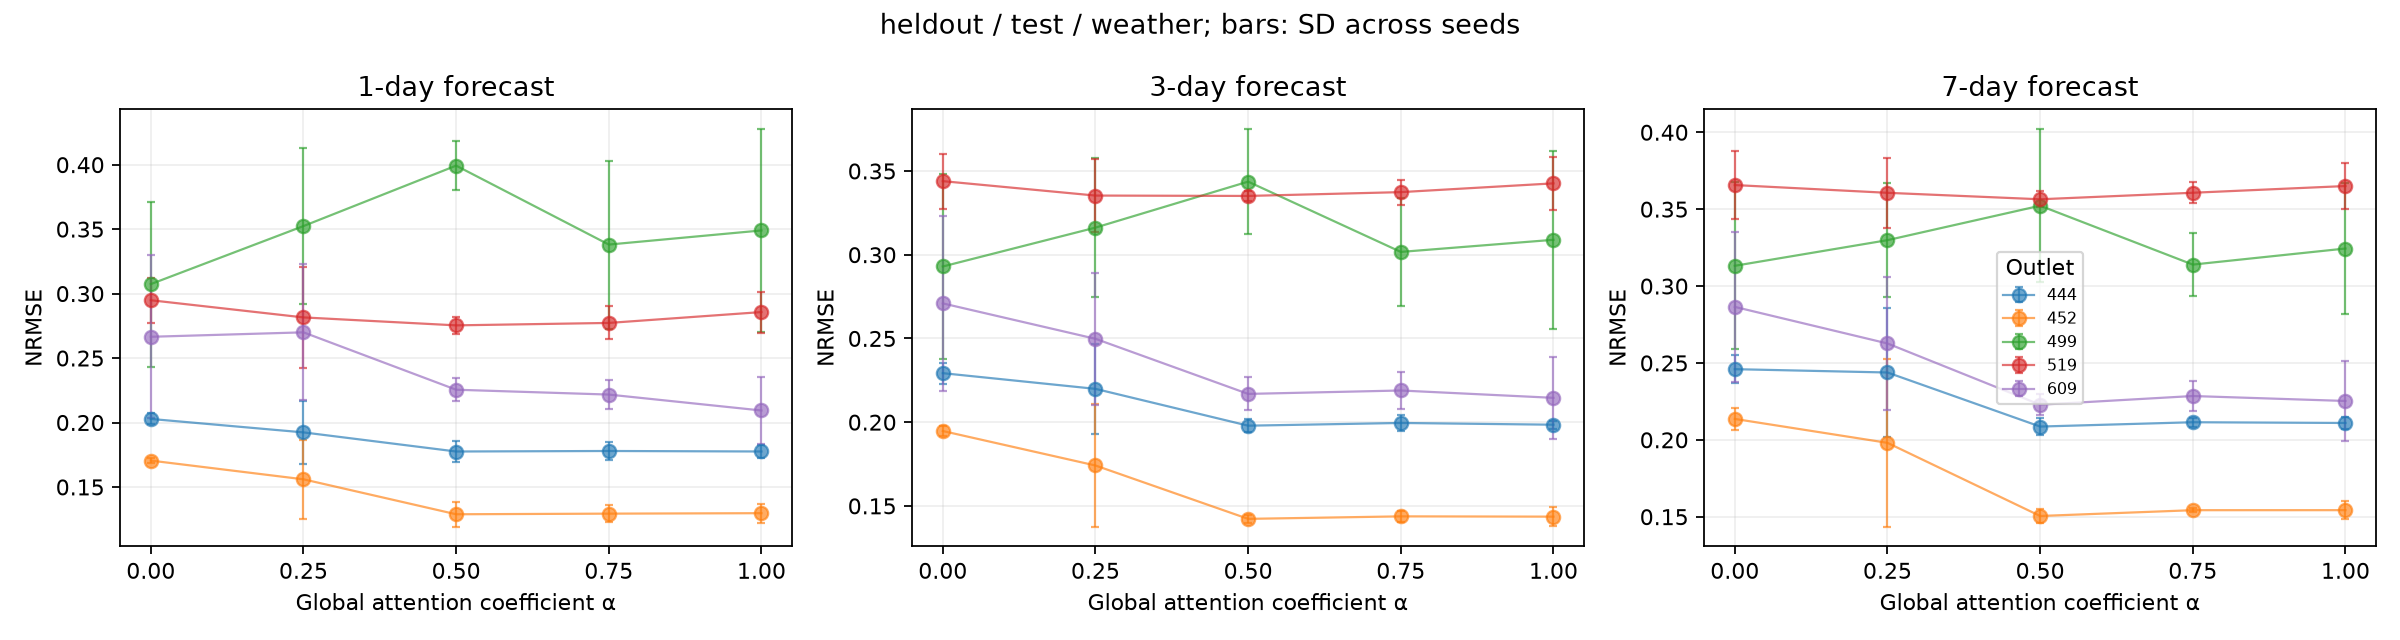
\includegraphics[width=0.85\textwidth]{river_alpha_curves_heldout_weather.png}\\[4pt]
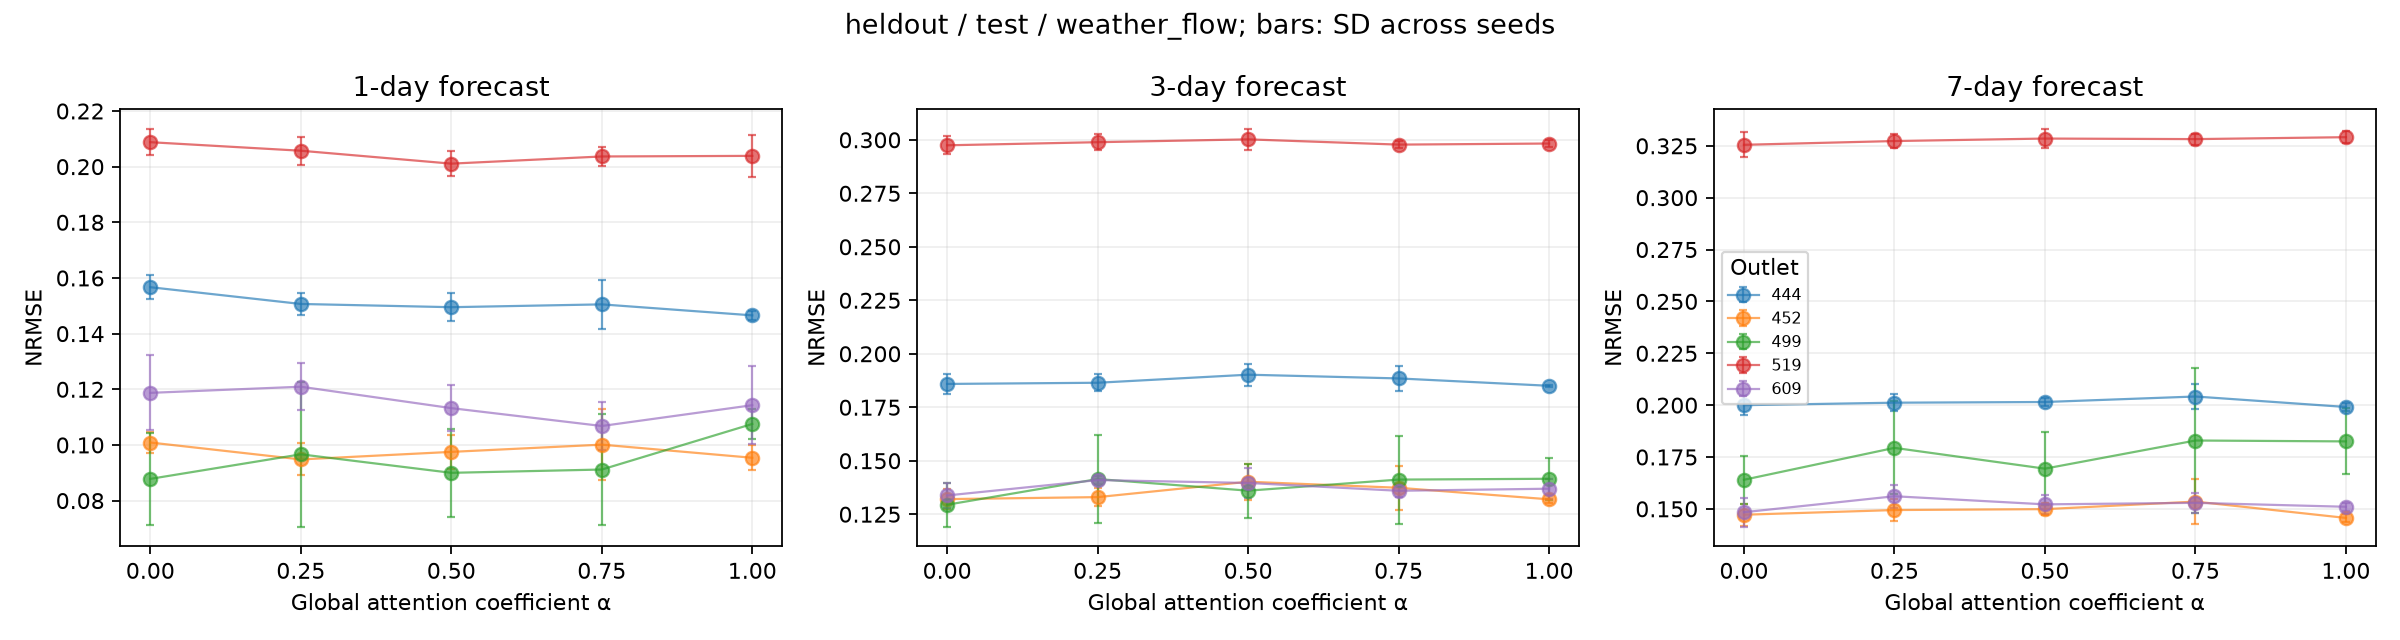
\includegraphics[width=0.85\textwidth]{river_alpha_curves_heldout_weather_flow.png}
\end{figure}

The context ablation tested whether the models used upstream information at all (Table~\ref{tab:context}). When dynamic inputs were hidden beyond the outlet itself, the error of the $\alpha=0.75$ blend rose by about 12\% and that of pure attention by about 13\%, so both exploited upstream context. Pure message passing behaved in the opposite way: it performed slightly better when upstream inputs were hidden than when they were available, on the development outlets as well as the held-out ones. A model that is better off without information it could in principle reach is consistent with over-squashing, although an optimisation effect, the mismatch between mean aggregation and the task, or the difference in parameter count could produce the same pattern. The ablation masks inputs and does not rewire the graph.

\begin{table}[htbp]
\caption{Held-out river test NRMSE under input-context ablation, weather inputs}
\label{tab:context}
\centering\small
\begin{tabular}{@{}lccc@{}}
\toprule
Configuration & Full context & Radius 2 & Radius 0 \\
\midrule
Message passing ($\alpha=0$) & 0.2666 & 0.2673 & \textbf{0.2584} \\
Hybrid, $\alpha=0.75$ & \textbf{0.2409} & 0.2695 & 0.2741 \\
Attention ($\alpha=1$) & \textbf{0.2426} & 0.2583 & 0.2791 \\
\bottomrule
\end{tabular}

\vspace{4pt}
\parbox{0.8\textwidth}{\footnotesize\textit{Note.} Radius $r$ keeps dynamic inputs only within $r$ hops of the outlet; static attributes and the graph are unchanged. Means over horizons and seeds.}
\end{table}

We tested whether upstream growth predicts the hybrid's benefit by relating each held-out outlet's two-hop volume $V(2)$ to the gain of the $\alpha=0.75$ blend (Table~\ref{tab:outlets} and Figure~\ref{fig:growthgain}). The outlet with the fastest growth, 499, gained least and was the only one made worse by the blend. The Spearman correlation between $V(2)$ and absolute gain was $-0.70$ at the 1- and 3-day horizons when the reference was message passing, but $+0.90$ at every horizon when the reference was attention, so the sign depended on the comparison. Leaving out one dependency group gave correlations spanning both signs, from $-1.0$ to $+0.5$ at the shorter horizons. Across the 27 development outlets, the association with gain over message passing in the weather regime was close to zero once size, depth and drainage area were taken into account, while other reference models and input regimes gave adjusted correlations between about $-0.27$ and $+0.37$. An existing graph-conditioned $\alpha$ selector, whose rules split on river length and mean branching, had a macro NRMSE of 0.212 against 0.207 for the validation-selected fixed $\alpha$, 2.3\% worse.

\begin{table}[htbp]
\caption{Gain of the $\alpha=0.75$ blend over message passing for each held-out outlet}
\label{tab:outlets}
\centering\small
\begin{tabular}{@{}rrrrrr@{}}
\toprule
Outlet & Nodes & Depth & $V(2)$ & Weather gain & Weather + flow gain \\
\midrule
444 & 9 & 6 & 3 & $+13.1\%$ & $-0.1\%$ \\
609 & 7 & 3 & 5 & $+18.8\%$ & $+1.3\%$ \\
452 & 8 & 3 & 6 & $+26.2\%$ & $-2.9\%$ \\
519 & 11 & 3 & 9 & $+2.9\%$ & $+0.3\%$ \\
499 & 29 & 7 & 13 & $-4.4\%$ & $-8.9\%$ \\
\bottomrule
\end{tabular}

\vspace{4pt}
\parbox{0.8\textwidth}{\footnotesize\textit{Note.} Positive values mean the blend has lower NRMSE than message passing. Seeds and horizons averaged first.}
\end{table}

\begin{figure}[htbp]
\caption{Two-hop upstream volume against gain of the $\alpha=0.75$ blend, held-out outlets, weather inputs, 3-day horizon}
\label{fig:growthgain}
\centering
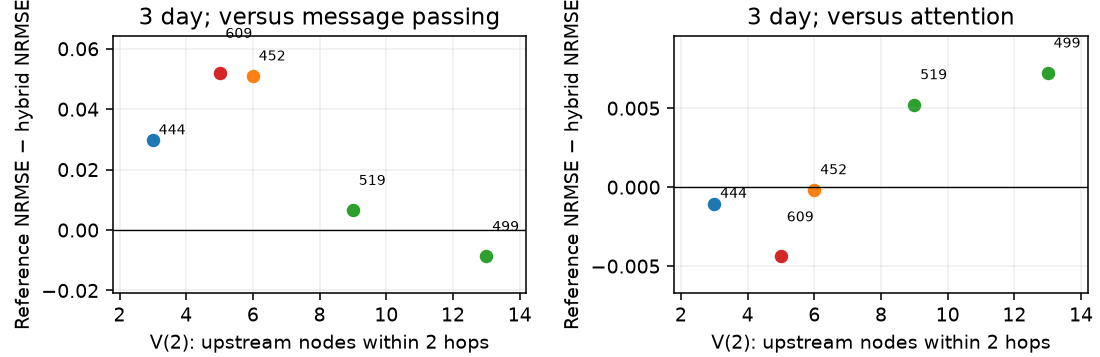
\includegraphics[width=0.7\textwidth]{river_growth_vs_gain_heldout_weather_a075_3day_mp_vs_attn.png}
\end{figure}

The hybrids were also the most expensive models (Figure~\ref{fig:cost}). A blend with both branches had about 491,000 active parameters and took about 80 seconds of training per epoch, against 53 to 54 seconds for either endpoint, while upstream pooling matched the best weather-only blend to within 1.1\% with about 27,000 parameters and 15 seconds per epoch. The full river study comprised 72 trained fits and about 28.5 hours of recorded training time.

\begin{figure}[htbp]
\caption{Training cost against $\alpha$ for the river models}
\label{fig:cost}
\centering
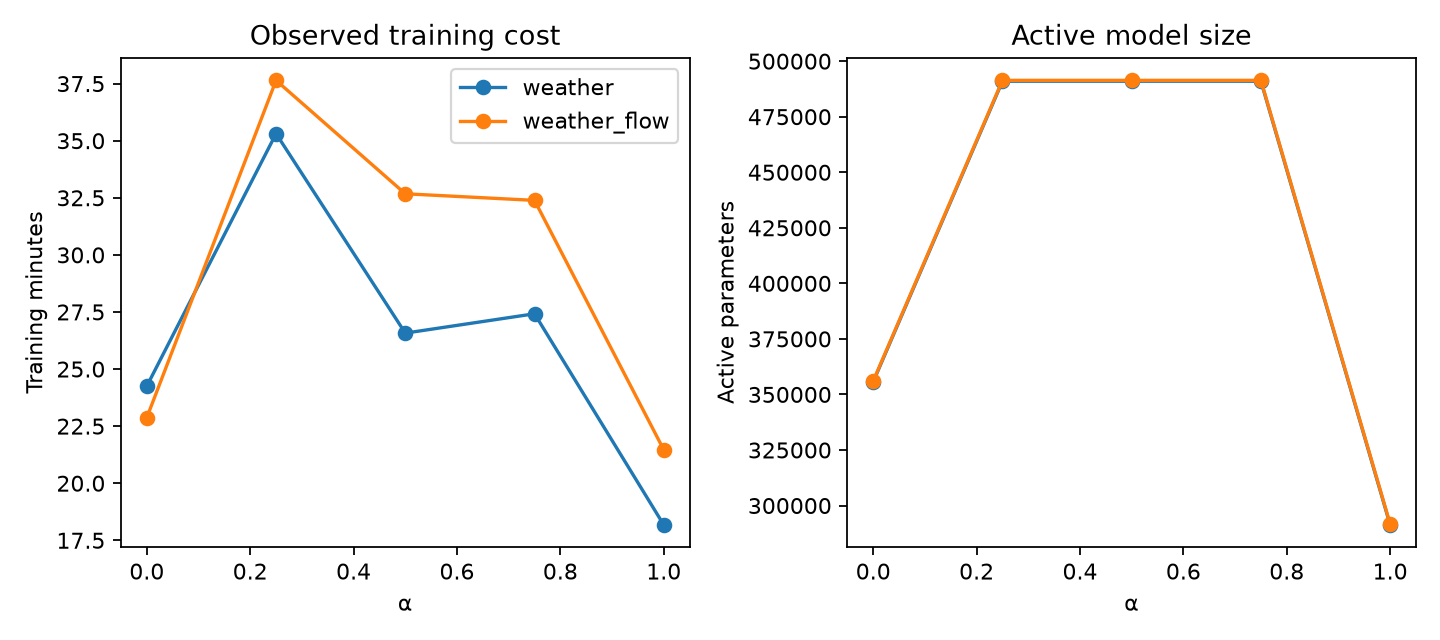
\includegraphics[width=0.7\textwidth]{river_cost_vs_alpha.png}
\end{figure}

\subsection{Controlled Tree Experiment}
On synthetic trees, both query distances lay inside the eight-layer receptive field of message passing, so a failure on the far query cannot be explained by reach alone. Table~\ref{tab:tree} shows that message passing answered the one-hop query almost perfectly but failed the four-hop query, with an MSE of 1.01, no better than predicting zero. Every blend solved both queries, and every blend was more accurate than pure attention on the balanced task. The validation-selected blend was $\alpha=0.25$.

\begin{table}[htbp]
\caption{Test MSE on the controlled tree task by query distance}
\label{tab:tree}
\centering\small
\begin{tabular}{@{}lccc@{}}
\toprule
Configuration & Near (1 hop) & Far (4 hops) & Balanced \\
\midrule
Message passing ($\alpha=0$) & 0.0036 & 1.0094 & 0.5065 \\
Hybrid, $\alpha=0.25$ & \textbf{0.0024} & 0.0129 & \textbf{0.0077} \\
Hybrid, $\alpha=0.50$ & 0.0074 & 0.0147 & 0.0110 \\
Hybrid, $\alpha=0.75$ & 0.0050 & \textbf{0.0122} & 0.0086 \\
Attention ($\alpha=1$) & 0.0093 & 0.0189 & 0.0141 \\
\bottomrule
\end{tabular}

\vspace{4pt}
\parbox{0.8\textwidth}{\footnotesize\textit{Note.} Predicting zero gives MSE 1; a topology-blind predictor gives 0.5. Means over seeds 42--44.}
\end{table}

\subsection{Pilot Results on Peptides-func and Reddit}
The pilot replication on Peptides-func used RWSE, 200 epochs with early-stopping patience 40, and one seed. The GPS model had four layers of width 96 (386,246 parameters) and the GCN six layers of width 240 with batch normalisation (412,790 parameters). GPS reached a test AP of 0.6518 (validation 0.6702), matching the published 0.6535 \citep{rampasek2022}, while the GCN reached 0.6263 (validation 0.6545), well short of the tuned value of about 0.686 reported by \citet{tonshoff2024}. The replication is therefore partial: it reproduces the hybrid but not the tuned message-passing baseline.

The pilot mechanistic notebook reported log-log Jacobian slopes against effective resistance of $-1.76$ for GINE, $-0.48$ for the graph transformer and $-0.81$ for GPS. Those models reached test AP of only 0.54, 0.27 and 0.24, so the attention models had not learned the task, and the setup had the flaws listed at the start of the Methodology. The entropy results were also narrower than the proposal stated: raw entropy rose with graph size for both attention models, but normalised entropy rose only for GPS ($r=+0.60$) and not for the transformer ($r=-0.09$). We therefore do not treat the pilot mechanistic results as evidence for H1 or H2; they are shown in Appendix~B for completeness.

The pilot Reddit experiment, averaged over 100 seeds, found that the virtual-master-node model reduced mean squared error relative to GraphSAGE by 12\%, 38\%, 51\%, 62\% and 81\% at one, two, three, four and five or more hops from the anchor (Figure~\ref{fig:reddit}). The growth of the reduction with distance is the pattern over-squashing predicts, but three flaws prevent that reading: only the virtual-node model had an input projection layer, the target was nearly a function of each node's own features, and the distance split confounds distance with distribution shift. The rebuilt Reddit experiment, which fixes all three, has been implemented and tested on synthetic graphs but not yet run on the real graph.

\begin{figure}[htbp]
\caption{Pilot Reddit test MSE by hop distance from the anchor, GraphSAGE against the virtual-master-node model (100 seeds)}
\label{fig:reddit}
\centering
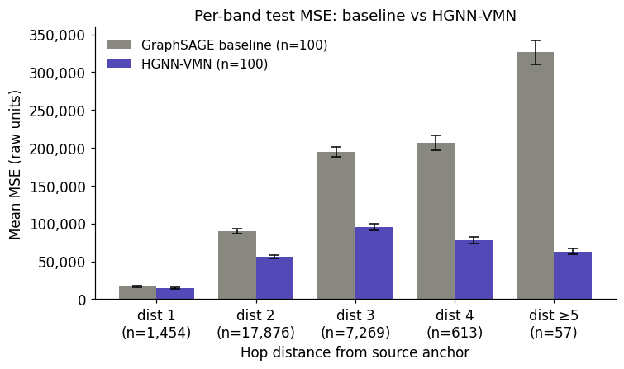
\includegraphics[width=0.72\textwidth]{proposal_image1.png}
\end{figure}

\subsection{Calibration of the Rebuilt Peptides Pipeline}
Gate G0 trained the rebuilt four-layer hybrid at $\alpha=0.5$ on a Colab T4 GPU. Training stopped early at epoch 182 after 40 epochs without improvement. The best validation AP was 0.6281 at epoch 142, where the test AP was 0.6259, which is 0.026 below the 0.652 threshold and below the G1 threshold of 0.63 that applies to the five-layer model. Figure~\ref{fig:g0} shows the logged training curve. Training loss fell monotonically from 0.152 at epoch 30 to 0.009, while validation AP rose to about 0.62 by epoch 90 and then stayed within 0.01 of that value; this pattern of continued fitting without validation gain indicates overfitting rather than underfitting. The calibration run took about 19 seconds per epoch.

\begin{figure}[htbp]
\caption{Gate G0 calibration run: training loss and validation AP of the rebuilt four-layer hybrid ($\alpha=0.5$, seed 0)}
\label{fig:g0}
\centering
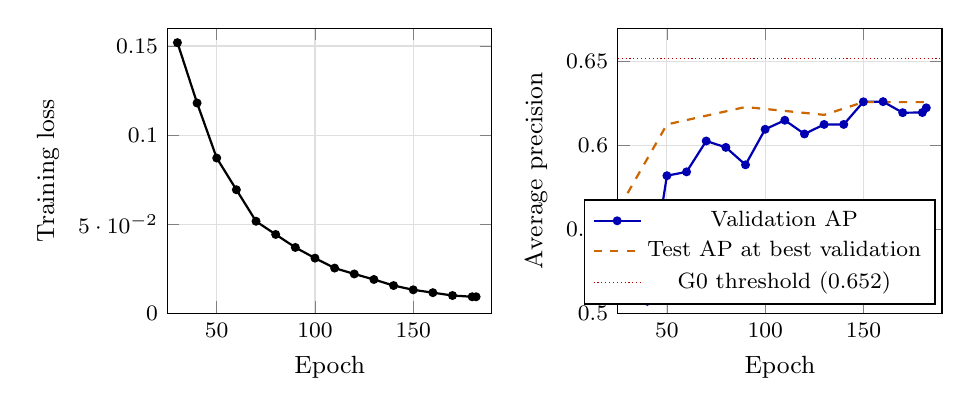
\begin{tikzpicture}
\begin{groupplot}[group style={group size=2 by 1, horizontal sep=1.6cm},
    width=0.47\textwidth, height=5.2cm, xlabel={Epoch}, xmin=25, xmax=190,
    tick label style={font=\footnotesize}, label style={font=\small},
    grid=major, grid style={gray!25}]
\nextgroupplot[ylabel={Training loss}, ymin=0, ymax=0.16]
\addplot[thick, color=black, mark=*, mark size=1.2pt] coordinates {
 (30,0.1519) (40,0.1180) (50,0.0871) (60,0.0693) (70,0.0516) (80,0.0442) (90,0.0369)
 (100,0.0309) (110,0.0253) (120,0.0220) (130,0.0189) (140,0.0155) (150,0.0131)
 (160,0.0115) (170,0.0099) (180,0.0092) (182,0.0092)};
\nextgroupplot[ylabel={Average precision}, ymin=0.50, ymax=0.67,
    legend style={font=\footnotesize, at={(0.98,0.03)}, anchor=south east}]
\addplot[thick, color=blue!70!black, mark=*, mark size=1.2pt] coordinates {
 (30,0.5475) (40,0.5071) (50,0.5820) (60,0.5843) (70,0.6027) (80,0.5989) (90,0.5885)
 (100,0.6097) (110,0.6151) (120,0.6069) (130,0.6126) (140,0.6126) (150,0.6261)
 (160,0.6262) (170,0.6196) (180,0.6197) (182,0.6225)};
\addlegendentry{Validation AP}
\addplot[thick, dashed, color=orange!80!black] coordinates {
 (30,0.5716) (50,0.6126) (90,0.6230) (130,0.6183) (150,0.6259) (182,0.6259)};
\addlegendentry{Test AP at best validation}
\addplot[thin, densely dotted, color=red!70!black, domain=25:190] {0.652};
\addlegendentry{G0 threshold (0.652)}
\end{groupplot}
\end{tikzpicture}

\vspace{4pt}
\parbox{0.9\textwidth}{\footnotesize\textit{Note.} Logged every 10 epochs from epoch 30; the first 20 epochs ran in an earlier Colab session. Test AP is a step function that changes only when validation AP reaches a new best.}
\end{figure}

The mechanistic measurements for this run did not complete. The Jacobian and entropy sweeps ran, but the graph-level Hessian range exhausted the T4's 15 GB of memory, fell back to a slower per-row computation, and was stopped before results were written. The sanity runs at $\alpha=0$ and $\alpha=1$ were started but had not finished at the time of writing, so gate G0 is not yet passed on either of its criteria.

\subsection{Behaviour of the Measures on Untrained Models}
As a check that the measures respond to the mechanisms they target, we applied them to untrained models built from the same code (Appendix~A). The message-passing model's sensitivity fell by a factor of about 3 to 10 per hop and was exactly zero beyond its $L$-hop receptive field; pure attention was flat at about $1/N$; and the $\alpha=0.5$ hybrid followed the local curve for two to three hops before settling on a floor about half as high. Attention entropy lay on $\log N$, with normalised entropy of at least 0.995, and the sensitivity of the global model to sources six or more hops away fell exactly as $1/N$, from $6.8\times10^{-2}$ at $N=16$ to $2.1\times10^{-3}$ at $N=512$. On a 150-node path the node-level range of the five-layer local model was 0.67 hops, within its receptive field, and grew to 18.7 hops for the hybrid and 34.3 hops for pure attention. These values describe untrained models and are not findings about trained ones.

% ================================================================
\section{Discussion}
The objectives were partly achieved. The measurement framework is complete and verified: each measure behaves as theory predicts on analytic cases and on untrained models, and the pipeline produces stratified, bootstrapped results from saved predictions. The empirical question, whether structure and task range predict the best $\alpha$, has been answered only on the river and tree data, and the main mechanistic study on Peptides is still waiting for a sound training regime.

The river and tree experiments agree on one point. Global access helps when the target depends on information that message passing does not deliver to the receiving node, and it helps little otherwise. In the weather-only river regime, the outlet's own weather says little about future discharge, upstream rainfall matters, and every model with global access beat message passing. Once the outlet's discharge history was supplied, local information sufficed, and the hybrid only added cost. In the tree task, message passing failed the far query even though the far nodes were within reach, while every blend succeeded. The context ablation, in which message passing did better with upstream inputs hidden, is the strongest real-data hint of an over-squashing-like failure, but it is not a diagnosis: mean aggregation, the attention-only hop bias, layer normalisation that strips amplitude, and unequal parameter counts all differed between the endpoints. These confounds are the reason a second tree experiment with a residual sum-aggregation model, matched parameter counts and no attention-only structural features has been designed.

The best model in each setting was not a blend. Pure attention and upstream pooling were within about 1\% of the best weather-only blend at lower cost, and pooling was best with flow history. Blends won on the controlled tree task, where they were more accurate than either endpoint. This suggests that a blend's value lies in robustness across query types rather than in a large advantage on any single task, which is consistent with H4 only in its weakest form. The growth hypothesis failed for identifiable reasons. Five held-out outlets in four dependency groups cannot support a correlation, the sign of the correlation flipped with the reference model, and graph size, depth and drainage area moved together. More seeds would not help, because seeds measure optimisation noise and do not add river networks.

The pilot Peptides evidence that the proposal relied on does not support the mechanistic hypotheses. Its Jacobian slopes came from attention models that did not train, its entropy rose with size only for GPS, and its Jacobians were taken through linear layers applied to categorical codes. On Peptides, effective resistance and hop distance are nearly collinear and both correlate with graph size, so even correct measurements there can show that sensitivity decays with distance but cannot separate resistance from distance. The rebuilt pipeline addresses the measurement flaws, and the transformer's slope is now used as a size-confound baseline rather than as evidence that attention bypasses bottlenecks.

The calibration result is the main open issue. The rebuilt hybrid fell short of the pilot GPS by 0.026 AP. The training curve points to overfitting, which makes dropout and normalisation the first changes to test, following the G1 procedure. A second possibility is that the rebuilt model is not equivalent to the pilot model in a way the calibration was meant to detect, such as the input encoding, the branch normalisation or the attention implementation; the pilot's validation AP of 0.670 against 0.628 here points the same way. Because the run used one seed, part of the gap may also be seed variance. The measurement failure has a direct remedy: the graph-level Hessian range is the least informative of the measures for comparing models, and it can be disabled or limited on a 15 GB GPU without affecting the Jacobian, entropy and node-level range results.

The study has further limitations. The $\alpha$ comparison changes the parameter count because unused branches are not built. The river model was not tuned exhaustively and its weather-only skill is below the mean-flow benchmark by the Nash--Sutcliffe criterion. The synthetic trees had unequal target draws across growth profiles, which can masquerade as a structural effect. All conclusions are limited to near-tree molecular graphs, river gauge trees, one social graph and synthetic rooted trees, and should not be extended to dense graphs or large-scale transformers.

% ================================================================
\section{Conclusion}
This project reframes graph architecture selection as the diagnosis of a binding constraint. The deliverable so far is a tested measurement package that computes, for any trained local, global or hybrid model, how its sensitivity decays with effective resistance, how concentrated its attention is, and how far its predictions reach, together with a resumable sweep and analysis pipeline that reports these quantities with graph-clustered confidence intervals. Applied to river forecasting and controlled trees, the framework showed that global access was worth 9.6\% in forecast error when distant information was needed and nothing when it was not, and that a simple measure of graph growth did not predict which case applied.

For a practitioner, the immediate recommendation is to test whether a task needs distant information before paying for global attention. A context-radius ablation of the kind used on the rivers is one inexpensive test. Where the test shows dependence on distant inputs, pure attention or simple upstream pooling should be tried alongside a hybrid, since in our results they came within about 1\% of the best hybrid at lower cost.

The next steps follow the project's phases. We will close the calibration gap by changing one factor at a time and rerun G0. We will then run the twelve-model Peptides-func re-baseline with Jacobian, entropy and range measurements, check gates G1 and G2, and run the rebuilt Reddit experiment with its random-split control. The $\alpha$ sweep will compare blends with a gated-attention baseline \citep{liu2026} and estimate the best $\alpha$ within effective-resistance bins. Comparing Peptides-func with Peptides-struct will measure whether range depends on the task on fixed graphs. A synthetic suite that varies effective resistance, long-range dependence and the number of distractor nodes independently will populate the phase diagram, and a simple predictor of best $\alpha$ from structure and range will be tested on held-out graphs. Beyond this project, the same measurements could be used to decide when to rewire a graph, when to add a virtual node, and when sparse attention is sufficient in other networked forecasting problems such as traffic and power grids.

% ================================================================
\newpage
\section{References}
\begingroup
\singlespacing
\setlength{\parindent}{0pt}
\renewcommand{\refname}{}
\renewcommand{\section}[2]{}%
\setlength{\bibsep}{10pt}
\setlength{\bibhang}{0.5in}
% APA 7 reference list, verified against arXiv, PMLR, NeurIPS proceedings, Crossref and TMLR.
% Labels are natbib author-year labels so \citep gives "(Alon & Yahav, 2021)".
\begin{thebibliography}{99}

\bibitem[Alon \& Yahav(2021)]{alon2021}
Alon, U., \& Yahav, E. (2021). On the bottleneck of graph neural networks and its practical implications. In \emph{International Conference on Learning Representations}. https://arxiv.org/abs/2006.05205

\bibitem[Bamberger et~al.(2025)]{bamberger2025}
Bamberger, J., Gutteridge, B., Le Roux, S., Bronstein, M. M., \& Dong, X. (2025). On measuring long-range interactions in graph neural networks. In \emph{Proceedings of the 42nd International Conference on Machine Learning} (Vol. 267, pp. 2770--2789). PMLR.

\bibitem[Black et~al.(2023)]{black2023}
Black, M., Wan, Z., Nayyeri, A., \& Wang, Y. (2023). Understanding oversquashing in GNNs through the lens of effective resistance. In \emph{Proceedings of the 40th International Conference on Machine Learning} (Vol. 202, pp. 2528--2547). PMLR.

\bibitem[Di~Giovanni et~al.(2023)]{digiovanni2023}
Di Giovanni, F., Giusti, L., Barbero, F., Luise, G., Li\`{o}, P., \& Bronstein, M. M. (2023). On over-squashing in message passing neural networks: The impact of width, depth, and topology. In \emph{Proceedings of the 40th International Conference on Machine Learning} (Vol. 202, pp. 7865--7885). PMLR.

\bibitem[Dwivedi \& Bresson(2021)]{dwivedi2021}
Dwivedi, V. P., \& Bresson, X. (2021). \emph{A generalization of transformer networks to graphs} [Paper presentation]. AAAI 2021 Workshop on Deep Learning on Graphs: Methods and Applications (DLG-AAAI 2021). https://arxiv.org/abs/2012.09699

\bibitem[Dwivedi et~al.(2022)]{dwivedi2022}
Dwivedi, V. P., Ramp\'{a}\v{s}ek, L., Galkin, M., Parviz, A., Wolf, G., Luu, A. T., \& Beaini, D. (2022). Long range graph benchmark. In \emph{Advances in Neural Information Processing Systems} (Vol. 35, pp. 22326--22340).

\bibitem[Gilmer et~al.(2017)]{gilmer2017}
Gilmer, J., Schoenholz, S. S., Riley, P. F., Vinyals, O., \& Dahl, G. E. (2017). Neural message passing for quantum chemistry. In \emph{Proceedings of the 34th International Conference on Machine Learning} (Vol. 70, pp. 1263--1272). PMLR.

\bibitem[Hamilton et~al.(2017)]{hamilton2017}
Hamilton, W. L., Ying, R., \& Leskovec, J. (2017). Inductive representation learning on large graphs. In \emph{Advances in Neural Information Processing Systems} (Vol. 30).

\bibitem[Hu et~al.(2020)]{hu2020}
Hu, W., Liu, B., Gomes, J., Zitnik, M., Liang, P., Pande, V., \& Leskovec, J. (2020). Strategies for pre-training graph neural networks. In \emph{International Conference on Learning Representations}.

\bibitem[Kipf \& Welling(2017)]{kipf2017}
Kipf, T. N., \& Welling, M. (2017). Semi-supervised classification with graph convolutional networks. In \emph{International Conference on Learning Representations}.

\bibitem[Klingler et~al.(2021)]{klingler2021}
Klingler, C., Schulz, K., \& Herrnegger, M. (2021). LamaH-CE: LArge-SaMple DAta for hydrology and environmental sciences for Central Europe. \emph{Earth System Science Data, 13}, 4529--4565. https://doi.org/10.5194/essd-13-4529-2021

\bibitem[Kratzert et~al.(2019)]{kratzert2019}
Kratzert, F., Klotz, D., Shalev, G., Klambauer, G., Hochreiter, S., \& Nearing, G. (2019). Towards learning universal, regional, and local hydrological behaviors via machine learning applied to large-sample datasets. \emph{Hydrology and Earth System Sciences, 23}(12), 5089--5110. https://doi.org/10.5194/hess-23-5089-2019

\bibitem[Kreuzer et~al.(2021)]{kreuzer2021}
Kreuzer, D., Beaini, D., Hamilton, W. L., L\'{e}tourneau, V., \& Tossou, P. (2021). Rethinking graph transformers with spectral attention. In \emph{Advances in Neural Information Processing Systems} (Vol. 34, pp. 21618--21629).

\bibitem[Kumar et~al.(2018)]{kumar2018}
Kumar, S., Hamilton, W. L., Leskovec, J., \& Jurafsky, D. (2018). Community interaction and conflict on the web. In \emph{Proceedings of the 2018 World Wide Web Conference} (pp. 933--943). https://doi.org/10.1145/3178876.3186141

\bibitem[Liu et~al.(2024)]{liu2024}
Liu, N. F., Lin, K., Hewitt, J., Paranjape, A., Bevilacqua, M., Petroni, F., \& Liang, P. (2024). Lost in the middle: How language models use long contexts. \emph{Transactions of the Association for Computational Linguistics, 12}, 157--173. https://doi.org/10.1162/tacl\_a\_00638

\bibitem[Liu et~al.(2026)]{liu2026}
Liu, Y., Guo, D., Zheng, T., Yiu, S. M., Ning, L., \& Wu, J. (2026). \emph{Capacity-controlled global attention for graph transformers} (arXiv:2604.17324). arXiv. https://doi.org/10.48550/arXiv.2604.17324

\bibitem[Loshchilov \& Hutter(2019)]{loshchilov2019}
Loshchilov, I., \& Hutter, F. (2019). Decoupled weight decay regularization. In \emph{International Conference on Learning Representations}.

\bibitem[Ma et~al.(2023)]{ma2023}
Ma, L., Lin, C., Lim, D., Romero-Soriano, A., Dokania, P. K., Coates, M., Torr, P., \& Lim, S.-N. (2023). Graph inductive biases in transformers without message passing. In \emph{Proceedings of the 40th International Conference on Machine Learning} (Vol. 202, pp. 23321--23337). PMLR.

\bibitem[Miglior et~al.(2025)]{miglior2025}
Miglior, L., Tolloso, M., Gravina, A., \& Bacciu, D. (2025). \emph{Can you hear me now? A benchmark for long-range graph propagation} (arXiv:2512.17762). arXiv. https://doi.org/10.48550/arXiv.2512.17762

\bibitem[Mishayev et~al.(2025)]{mishayev2025}
Mishayev, Y., Sverdlov, Y., Amir, T., \& Dym, N. (2025). \emph{Short-range oversquashing} (arXiv:2511.20406). arXiv. https://doi.org/10.48550/arXiv.2511.20406

\bibitem[Nash \& Sutcliffe(1970)]{nash1970}
Nash, J. E., \& Sutcliffe, J. V. (1970). River flow forecasting through conceptual models part I---A discussion of principles. \emph{Journal of Hydrology, 10}(3), 282--290. https://doi.org/10.1016/0022-1694(70)90255-6

\bibitem[Ramp\'{a}\v{s}ek et~al.(2022)]{rampasek2022}
Ramp\'{a}\v{s}ek, L., Galkin, M., Dwivedi, V. P., Luu, A. T., Wolf, G., \& Beaini, D. (2022). Recipe for a general, powerful, scalable graph transformer. In \emph{Advances in Neural Information Processing Systems} (Vol. 35, pp. 14501--14515).

\bibitem[Shirzad et~al.(2023)]{shirzad2023}
Shirzad, H., Velingker, A., Venkatachalam, B., Sutherland, D. J., \& Sinop, A. K. (2023). Exphormer: Sparse transformers for graphs. In \emph{Proceedings of the 40th International Conference on Machine Learning} (Vol. 202, pp. 31613--31632). PMLR.

\bibitem[Sun et~al.(2025)]{sun2025}
Sun, J., Chang, W., Yang, C., Huang, Q., \& Wang, S. (2025). Relieving the over-aggregating effect in graph transformers. In \emph{Advances in Neural Information Processing Systems} (Vol. 38, pp. 6673--6699).

\bibitem[T\"{o}nshoff et~al.(2024)]{tonshoff2024}
T\"{o}nshoff, J., Ritzert, M., Rosenbluth, E., \& Grohe, M. (2024). Where did the gap go? Reassessing the long-range graph benchmark. \emph{Transactions on Machine Learning Research}. https://openreview.net/forum?id=Nm0WX86sKv

\bibitem[Topping et~al.(2022)]{topping2022}
Topping, J., Di Giovanni, F., Chamberlain, B. P., Dong, X., \& Bronstein, M. M. (2022). Understanding over-squashing and bottlenecks on graphs via curvature. In \emph{International Conference on Learning Representations}.

\bibitem[Vaswani et~al.(2017)]{vaswani2017}
Vaswani, A., Shazeer, N., Parmar, N., Uszkoreit, J., Jones, L., Gomez, A. N., Kaiser, \L{}., \& Polosukhin, I. (2017). Attention is all you need. In \emph{Advances in Neural Information Processing Systems} (Vol. 30).

\bibitem[Xing et~al.(2024)]{xing2024}
Xing, Y., Wang, X., Li, Y., Huang, H., \& Shi, C. (2024). Less is more: On the over-globalizing problem in graph transformers. In \emph{Proceedings of the 41st International Conference on Machine Learning} (Vol. 235, pp. 54656--54672). PMLR.

\bibitem[Xu et~al.(2019)]{xu2019}
Xu, K., Hu, W., Leskovec, J., \& Jegelka, S. (2019). How powerful are graph neural networks? In \emph{International Conference on Learning Representations}.

\bibitem[Ying et~al.(2021)]{ying2021}
Ying, C., Cai, T., Luo, S., Zheng, S., Ke, G., He, D., Shen, Y., \& Liu, T.-Y. (2021). Do transformers really perform badly for graph representation? In \emph{Advances in Neural Information Processing Systems} (Vol. 34, pp. 28877--28888).

% New references for the front half (Abstract to Methodology). APA 7, natbib author-year labels.
% Keys are prefixed f_ so they cannot clash with the back-half references.
% Already in references.tex and reused: miglior2025 (ECHO), ying2021 (Graphormer), kumar2018 (Reddit),
% bamberger2025, black2023, tonshoff2024, xing2024, sun2025, rampasek2022, ...
% Input inside the thebibliography environment (these are \bibitem lines only).

\bibitem[Abboud et~al.(2022)]{f_abboud2022}
Abboud, R., Dimitrov, R., \& Ceylan, \.{I}. \.{I}. (2022). Shortest path networks for graph property prediction. In \emph{Proceedings of the First Learning on Graphs Conference} (Vol. 198). PMLR. https://arxiv.org/abs/2206.01003

\bibitem[Choromanski et~al.(2021)]{f_choromanski2021}
Choromanski, K., Likhosherstov, V., Dohan, D., Song, X., Gane, A., Sarlos, T., Hawkins, P., Davis, J., Mohiuddin, A., Kaiser, \L{}., Belanger, D., Colwell, L., \& Weller, A. (2021). Rethinking attention with Performers. In \emph{International Conference on Learning Representations}. https://arxiv.org/abs/2009.14794

\bibitem[De~Domenico et~al.(2013)]{f_dedomenico2013}
De Domenico, M., Lima, A., Mougel, P., \& Musolesi, M. (2013). The anatomy of a scientific rumor. \emph{Scientific Reports, 3}, 2980. https://doi.org/10.1038/srep02980

\bibitem[Eremeev et~al.(2026)]{f_eremeev2026}
Eremeev, D., Platonov, O., Bazhenov, G., Babenko, A., \& Prokhorenkova, L. (2026). GraphPFN: A prior-data fitted graph foundation model. In \emph{Proceedings of the 43rd International Conference on Machine Learning}. https://arxiv.org/abs/2509.21489

\bibitem[Gutteridge et~al.(2023)]{f_gutteridge2023}
Gutteridge, B., Dong, X., Bronstein, M. M., \& Di Giovanni, F. (2023). DRew: Dynamically rewired message passing with delay. In \emph{Proceedings of the 40th International Conference on Machine Learning} (Vol. 202). PMLR. https://arxiv.org/abs/2305.08018

\bibitem[Gutteridge et~al.(2026)]{f_gutteridge2026}
Gutteridge, B., Bronstein, M. M., \& Dong, X. (2026). \emph{Can graph foundation models generalize over architecture?} (arXiv:2603.22984). arXiv. https://doi.org/10.48550/arXiv.2603.22984

\bibitem[Ioffe \& Szegedy(2015)]{f_ioffe2015}
Ioffe, S., \& Szegedy, C. (2015). Batch normalization: Accelerating deep network training by reducing internal covariate shift. In \emph{Proceedings of the 32nd International Conference on Machine Learning} (Vol. 37, pp. 448--456). PMLR.

\bibitem[Karypis \& Kumar(1998)]{f_karypis1998}
Karypis, G., \& Kumar, V. (1998). A fast and high quality multilevel scheme for partitioning irregular graphs. \emph{SIAM Journal on Scientific Computing, 20}(1), 359--392. https://doi.org/10.1137/S1064827595287997

\bibitem[Lee et~al.(2026)]{f_lee2026}
Lee, J., Lee, D., Jeong, M., \& Yoo, J. (2026). \emph{NodeGround: A node classification benchmark in the graph foundation model era} (arXiv:2609.39673). arXiv. https://doi.org/10.48550/arXiv.2609.39673

\bibitem[Leskovec \& Krevl(2014)]{f_leskovec2014}
Leskovec, J., \& Krevl, A. (2014). \emph{SNAP Datasets: Stanford large network dataset collection} [Data set]. http://snap.stanford.edu/data

\bibitem[McPherson et~al.(2001)]{f_mcpherson2001}
McPherson, M., Smith-Lovin, L., \& Cook, J. M. (2001). Birds of a feather: Homophily in social networks. \emph{Annual Review of Sociology, 27}, 415--444. https://doi.org/10.1146/annurev.soc.27.1.415

\bibitem[Rozemberczki et~al.(2021)]{f_rozemberczki2021}
Rozemberczki, B., Allen, C., \& Sarkar, R. (2021). Multi-scale attributed node embedding. \emph{Journal of Complex Networks, 9}(2), cnab014. https://doi.org/10.1093/comnet/cnab014

\bibitem[Rozemberczki \& Sarkar(2021)]{f_rozemberczki2021b}
Rozemberczki, B., \& Sarkar, R. (2021). \emph{Twitch gamers: A dataset for evaluating proximity preserving and structural role-based node embeddings} (arXiv:2101.03091). arXiv. https://doi.org/10.48550/arXiv.2101.03091

\bibitem[von Luxburg et~al.(2014)]{f_vonluxburg2014}
von Luxburg, U., Radl, A., \& Hein, M. (2014). Hitting and commute times in large random neighborhood graphs. \emph{Journal of Machine Learning Research, 15}, 1751--1798.

\bibitem[Watts \& Strogatz(1998)]{f_watts1998}
Watts, D. J., \& Strogatz, S. H. (1998). Collective dynamics of `small-world' networks. \emph{Nature, 393}(6684), 440--442. https://doi.org/10.1038/30918

\end{thebibliography}

\endgroup

% ================================================================
\newpage
\appendixsection{A}{Mechanism Checks on Untrained Models}
The figures in this appendix use untrained models built from the same code as the trained ones and serve only to show that each measure responds to the mechanism it targets.

\begin{figure}[H]
\caption{Jacobian sensitivity against hop distance for untrained local, hybrid and global models}
\label{fig:demojac}
\centering
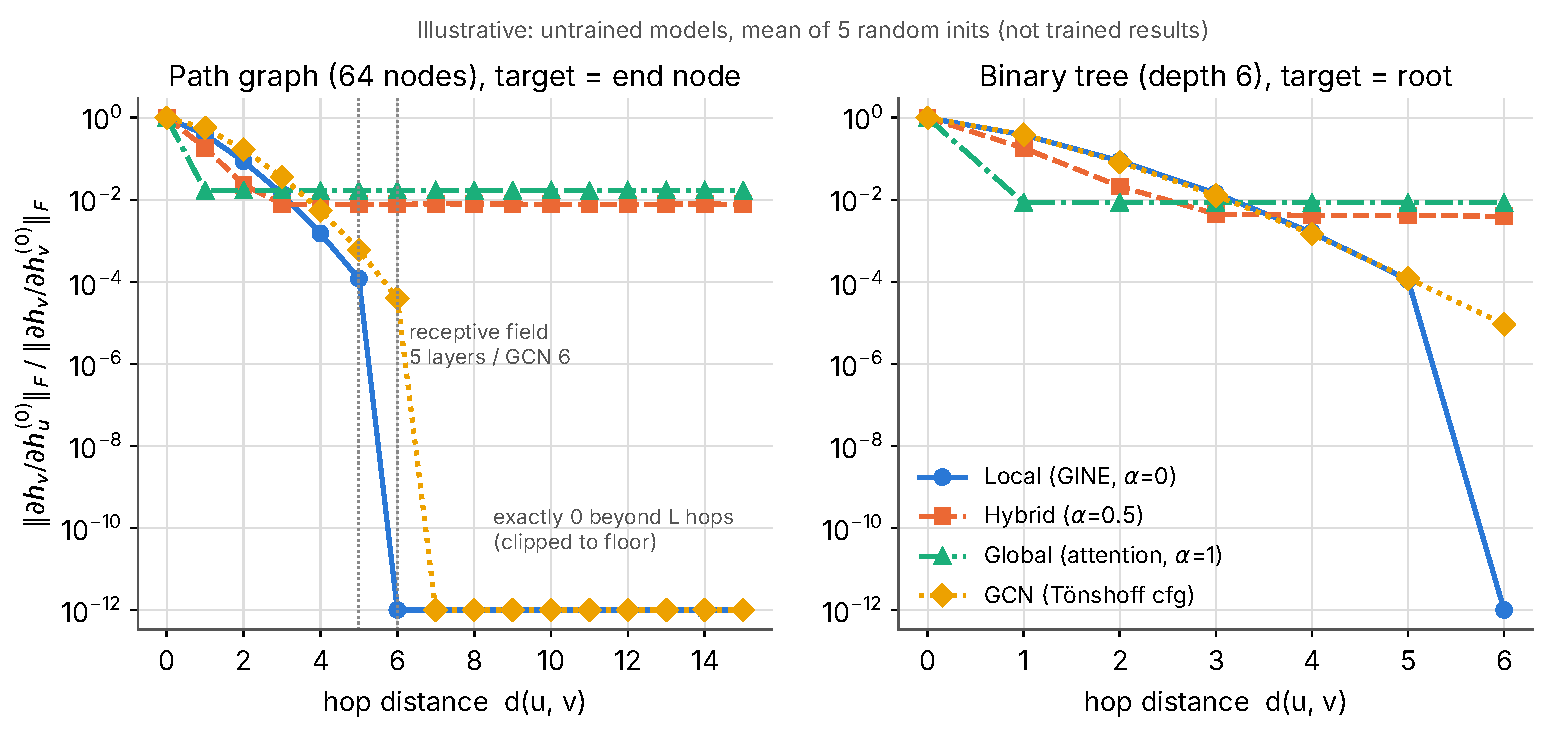
\includegraphics[width=0.85\textwidth]{demo_jacobian_vs_hops_untrained.pdf}
\end{figure}

\begin{figure}[H]
\caption{Attention entropy and long-range sensitivity against graph size for untrained attention models}
\label{fig:demoent}
\centering
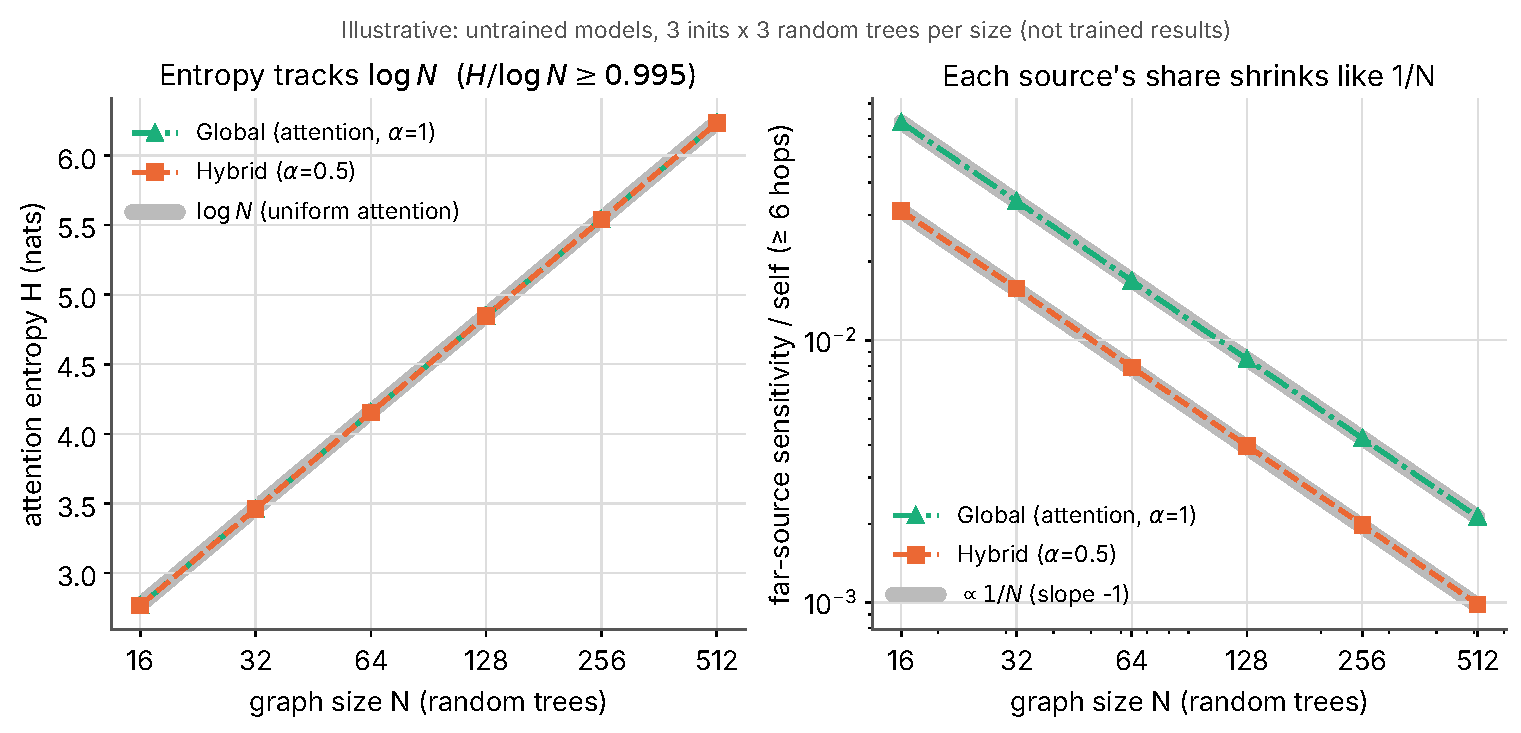
\includegraphics[width=0.85\textwidth]{demo_attention_dilution_untrained.pdf}
\end{figure}

\begin{table}[H]
\caption{Range measure on a 150-node path graph for untrained models}
\label{tab:demorange}
\centering\small
\begin{tabular}{@{}lcc@{}}
\toprule
Model & Node-level range, hops (mean / max) & Graph-level Hessian range \\
\midrule
Local, $\alpha=0$ (5 layers) & 0.67 / 0.69 & Undefined (ReLU only) \\
Hybrid, $\alpha=0.5$ & 18.7 / 25.8 & Not computed \\
Global, $\alpha=1$ & 34.3 / 47.0 & Not computed \\
GCN (6 layers, GELU) & 0.89 / 0.89 & 17.7 \\
\bottomrule
\end{tabular}
\end{table}

\appendixsection{B}{Pilot Mechanistic Results}
The pilot results below were produced before the pipeline was rebuilt. Models were trained for 30 epochs on one seed, atom codes were passed through a linear layer, no positional encoding was used, and entropy was computed on head-averaged attention. The test AP of each model is reported because a mechanism measured on a model that has not learned the task is not interpretable.

\begin{table}[H]
\caption{Pilot Jacobian slopes against effective resistance and test AP}
\label{tab:pilotjac}
\centering\small
\begin{tabular}{@{}lccc@{}}
\toprule
 & GINE & Graph transformer & GPS \\
\midrule
Log-log slope $b$ & $-1.76$ & $-0.48$ & $-0.81$ \\
Correlation $r$ & $-0.78$ & $-0.41$ & $-0.69$ \\
Test AP & 0.54 & 0.27 & 0.24 \\
\bottomrule
\end{tabular}
\end{table}

\begin{figure}[H]
\caption{Pilot Jacobian sensitivity against effective resistance by architecture}
\label{fig:pilotjac}
\centering
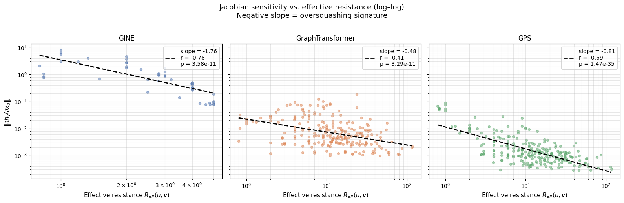
\includegraphics[width=\textwidth]{proposal_image3.png}
\end{figure}

\begin{figure}[H]
\caption{Pilot raw and normalised attention entropy against graph size}
\label{fig:pilotent}
\centering
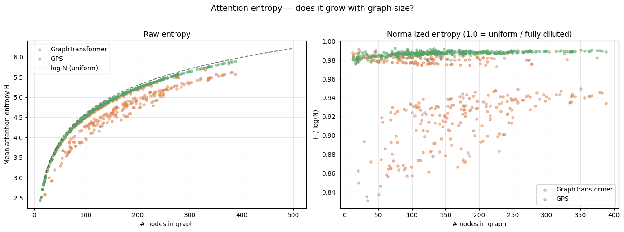
\includegraphics[width=\textwidth]{proposal_image4.png}
\end{figure}

\appendixsection{C}{Model Configurations}
\begin{table}[H]
\caption{Peptides-func model configurations and parameter counts}
\label{tab:configs}
\centering\small
\begin{tabular}{@{}lccccr@{}}
\toprule
Configuration & Hidden & Layers & Heads & Epochs & Parameters \\
\midrule
Local, $\alpha=0$ (GINE) & 96 & 5 & -- & 200 & 311,055 \\
Hybrid, $\alpha=0.5$ & 96 & 5 & 4 & 200 & 498,255 \\
Global, $\alpha=1$ (transformer) & 96 & 5 & 4 & 200 & 404,170 \\
GCN (aligned with T\"{o}nshoff et al.) & 235 & 6 & -- & 250 & 491,865 \\
G0 calibration, $\alpha=0.5$ & 96 & 4 & 4 & 200 & 404,654 \\
\bottomrule
\end{tabular}

\vspace{4pt}
\parbox{0.85\textwidth}{\footnotesize\textit{Note.} All models use RWSE with 20 steps, dropout 0.1, AdamW with learning rate $10^{-3}$ and five warm-up epochs. The benchmark budget is 500,000 parameters.}
\end{table}

\begin{table}[H]
\caption{River model parameter counts and training time per epoch}
\label{tab:rivercost}
\centering\small
\begin{tabular}{@{}lrr@{}}
\toprule
Model & Active parameters & Training seconds per epoch \\
\midrule
Message passing ($\alpha=0$) & 355,715 & 52.9 \\
Hybrid ($0<\alpha<1$) & 490,979 & 80.1--80.6 \\
Attention ($\alpha=1$) & 291,299 & 54.2 \\
Upstream pooling & 26,627 & 15.0 \\
Outlet-only GRU & 22,403 & 10.7 \\
\bottomrule
\end{tabular}

\vspace{4pt}
\parbox{0.85\textwidth}{\footnotesize\textit{Note.} Every configuration instantiates 490,979 parameters; the endpoints use only the active branch. Times exclude evaluation, on an RTX 3080 Laptop GPU.}
\end{table}

\end{document}
